\section{Реализация}

В этой главе я бы хотел порассуждать об архитектуре, через которую будет реализованно решение. На мой взгляд, очень часто ей уделяют недостаточно внимания. В то же время, от правильного планирования и реализации структуры проекта зависит его будущее. В моей практике встречается большое количество случаев, когда без своевременного продумывания архитектуры, компании годами сталкиваются с серьезными проблемами при поддержке и развитии легаси-кода.

\subsection{Общие соображения}
Как обычно выстраивается рабочий процесс, когда речь заходит о решении задачи по машинному обучению? В первую очередь в голову приходит довольно примитивная схема: есть некоторый пулл данных, для которых известен ответ (\textbf{Train}) и пулл, ответ для которого нужно предсказать (\textbf{ToPredict}). Мы загружаем первые данные в модель, обучаем ее, а затем получаем предсказание для данных второго типа. Представим эти соображения в виде схемы:

\begin{center} 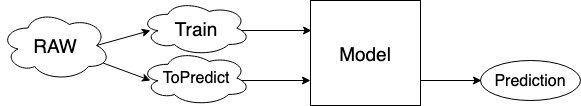
\includegraphics[width=350pt]{images/workflow_scheme_1}\end{center}

Следующим логическим развитием идеи будет добавление новой сущности для оценки качества модели (\textbf{ScoreCalculator}) и разделения известных данных на обучающие и тестовые (\textbf{Test}):


\begin{center} 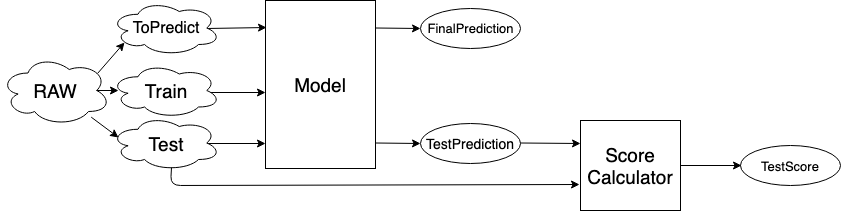
\includegraphics[width=450pt]{images/workflow_schema_2}\end{center}
Зачастую, с некоторыми небольшими вариациями, на этой схеме останавливаются. Мы же пройдем немного дальше.  Углубимся в детали, добавим некоторый новый расширяющий возможности функционал и постараемся сделать такую систему, которая бы легко масштабировалась на другие проекты, никак не связанные с нашей исходной задачей. 

\subsection{Усложняем структуру}
    
    В более сложных задачах данные требуют некоторой обработки (например, фильтрация, семплирование или преобразование в совершенно другую форму). Давайте в нашей диаграмме разделим данные на \textbf{XData},  \textbf{YData} и добавим сущность под названием \textbf{XTransformer}:
    
    \begin{center} 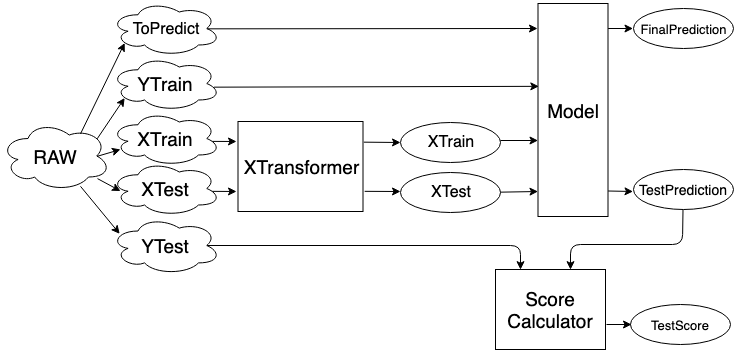
\includegraphics[width=450pt]{images/workflow_schema_3}\end{center}
    
    Еще одним нововведением предлагаю сделать сущность, которая бы отвечала за работу с сырыми данными: считывала, объединяла разные источники, разделяла на нужные выборки в нужном соотношении. Назовем ее \textbf{DataProvider}. По своему опыту могу судить о том, что такая инкапсуляция - одна из первых вещей, с которых стоит начинать развитие любого проекта, т.к. она освобождает основные алгоритмические сущности от управлением данных.
    
    \begin{center} 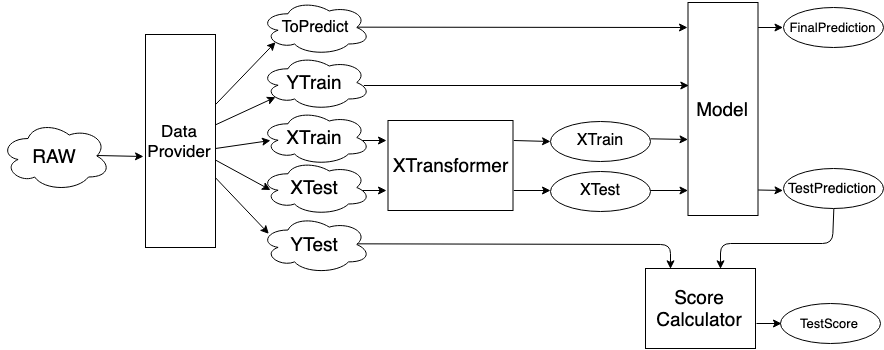
\includegraphics[width=450pt]{images/workflow_schema_4}\end{center}

    И завершающим элементом будет \textbf{Launcher} - точка входа в программу, которая является связующим звеном и реализует все связи, отображенные на схеме.
    
    
    \begin{center} 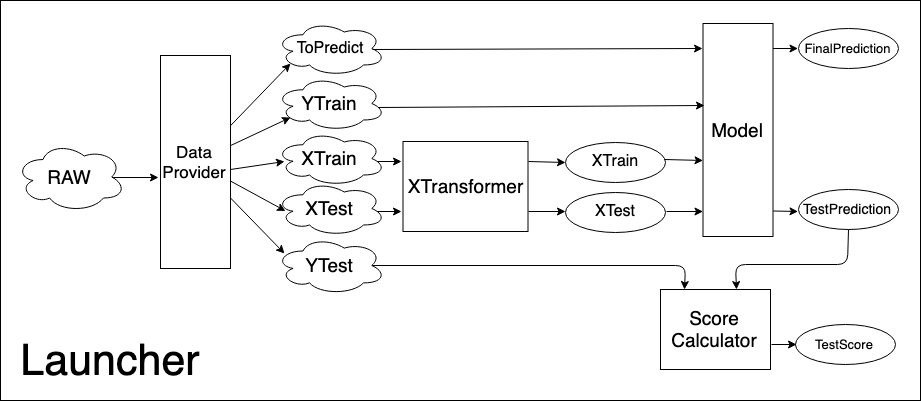
\includegraphics[width=450pt]{images/workflow_schema_5}\end{center}
    
    \pagebreak
    Выделим основные особенности архитектуры, которую мы получили:
    
    \begin{itemize}
        \item Не зависит от задачи, которая решается
        \item Состоит из независимых модулей, каждый из которых прост в реализации и решает одну определенную задачу
        \item Благодаря модульности, позволяет перебирать различные модели и трансформеры данных, чтобы подобрать оптимальные
        \item Легко добавить новые сущности, такие как композицию дополнительных моделей или визуализатор
    \end{itemize}
    
    
\pagebreak
\subsection{Техническая часть}
    
    В качестве языка программирования, на котором будет написан проект, очевидным выбором стал Python. Я начал с того, что в отдельном git репозитории реализовал структуру-каркас будущего решения, чтобы можно было взглянуть на разработанную архитектуру вне контекста решения задачи от Quora.
    
    Весь исходный код можно найти здесь: https://github.com/evgenstf/ml\_workflow.
    
    В рамках статьи мы не будем вдаваться в глубокие детали реализации, приведем лишь пару моментов, на которые стоит обратить внимание:
    
    \begin{itemize}
        \item \textbf{JSON конфиги}
        
     Всегда есть огромное количество констант, с которыми необходимо работать. От путей до данных и соотношения train/test до глубины решающего дерева и коэффициентов регуляризации. Мы будем держать их всех в одном месте: \textbf{config.json}, рядом с \textbf{launcher.py}. Для пустой реализации выглядит он следующим образом:
   \begin{lstlisting}[language=JSON]
{
  "data_provider": {
    "x_known": "../qdata/raw/simple_csv.csv",
    "y_known": "../qdata/raw/simple_csv.csv",
    "x_to_predict": "../qdata/raw/simple_csv.csv",
    "known_using_part" : 0.01, "train_part": 0.7
  },
  "x_transformer": {
    "name": "dummy"
  },
  "model": {
    "name": "dummy"
  },
  "answer_file": "answer.csv"
}
\end{lstlisting}

\pagebreak
    \item \textbf{Логгирование}
    
    Важнейшим аспектом разработки любого продукта является создание исчерпывающей системы логгирования. Мы будем поддерживать два режима: \textbf{DEBUG} и \textbf{INFO}.
    
    Ознакомиться с полным перечнем общеиспользуемых уровней логгирования и прочитать кейсы их применения можно вот здесь: \href{https://stackoverflow.com/questions/2031163/when-to-use-the-different-log-levels}{stackoverflow}.
    
    Пример информационного лога, который получается при запуске решения:
    \begin{lstlisting}[language=LOG]
INFO:Launcher:launcher config: {'x_transformer': {'name': 'w2v'}, 'model': {'loss_function': 'RMSE', 'l2_leaf_reg': 0.07, 'name': 'regboost', 'iterations': 1000, 'depth': 8, 'bootstrap_type': 'No', 'learning_rate': 0.2, 'classes_count': 5}, 'data_provider': {'x_to_predict': '../input/test.csv', 'known_using_part': 0.01, 'train_part': 0.8, 'x_known': '../input/train.csv', 'y_known': '../input/train.csv'}, 'embedding_provider': {'paragram_path': '../input/embeddings/paragram_300_sl999/paragram_300_sl999.txt', 'wiki_news_path': '../input/embeddings/wiki-news-300d-1M/wiki-news-300d-1M.vec', 'glove_path': '../input/embeddings/glove.840B.300d/glove.840B.300d.txt'}, 'answer_file': 'submission.csv'}
INFO:DataProvider:data provider config: {'x_to_predict': '../input/test.csv', 'known_using_part': 0.01, 'train_part': 0.8, 'x_known': '../input/train.csv', 'y_known': '../input/train.csv'}
INFO:DataProvider:loaded 13061 x_known lines
INFO:DataProvider:loaded 13061 y_known lines
INFO:DataProvider:loaded 56370 x_to_predict lines
INFO:DataProvider:splitted known data: x_train size: 10448 y_train size: 10448 x_test size: 2613 y_test size: 2613
INFO:DataProvider:inited
INFO:W2VXTransformer:x_transformer config:
INFO:W2VXTransformer:inited
INFO:W2VXTransformer:lemmatize called
\end{lstlisting}
    
	\end{itemize}
	
\subsection{Используемые библиотеки}

\subsubsection{Технические}

\begin{itemize}
    \item \textbf{json} - работа с JSON конфигами
    \item \textbf{logging} - логгирование
    \item \textbf{sys} - системные утилиты, такие как создание файлов, импорт из других дирикторий и т.п.
    \item \textbf{numpy} - упорядочивание данных, статистики, представления в виде таблиц
    \item \textbf{pandas} - надстройка над \textbf{numpy}, имеет в своем арсенале более продвинутые инструменты для исследований
    \item \textbf{sclearn} - набор метрик, инструменты для разделения данных на \textbf{train} и \textbf{test}
    \item \textbf{tqdm} - строка состояния обработки данных
\end{itemize}

\subsubsection{Препроцессинг}
\begin{itemize}
    \item \textbf{spacy} - инструменты для лемматизации и стеммизации слов
\end{itemize}


\subsubsection{Модель}
\begin{itemize}
    \item \textbf{keras.layers.LSTM} - реализация LSTM из библиотеки \textbf{keras}
    \item \textbf{keras.layers.Embedding} - работа с матрицей векторизации слов
    \item \textbf{keras.layers.Dropout} - реализация алгоритма \textbf{Dropout}, при котором удаляются случайные связи в сети для уменьшения переобучения.
    \item \textbf{keras.layers.Bidirectional} - бинаправленность в сети
\end{itemize}


\subsection{Результаты}

Лучший результат по F - мере, который мне удалось достичь используя векторизацию и LSTM - \textbf{0.63}. Можно сказать, что это скорее удачный результат, поскольку он показывает себя лучше, чем 70\% участников соревнования. 




